\begin{figure}[H]
\centering
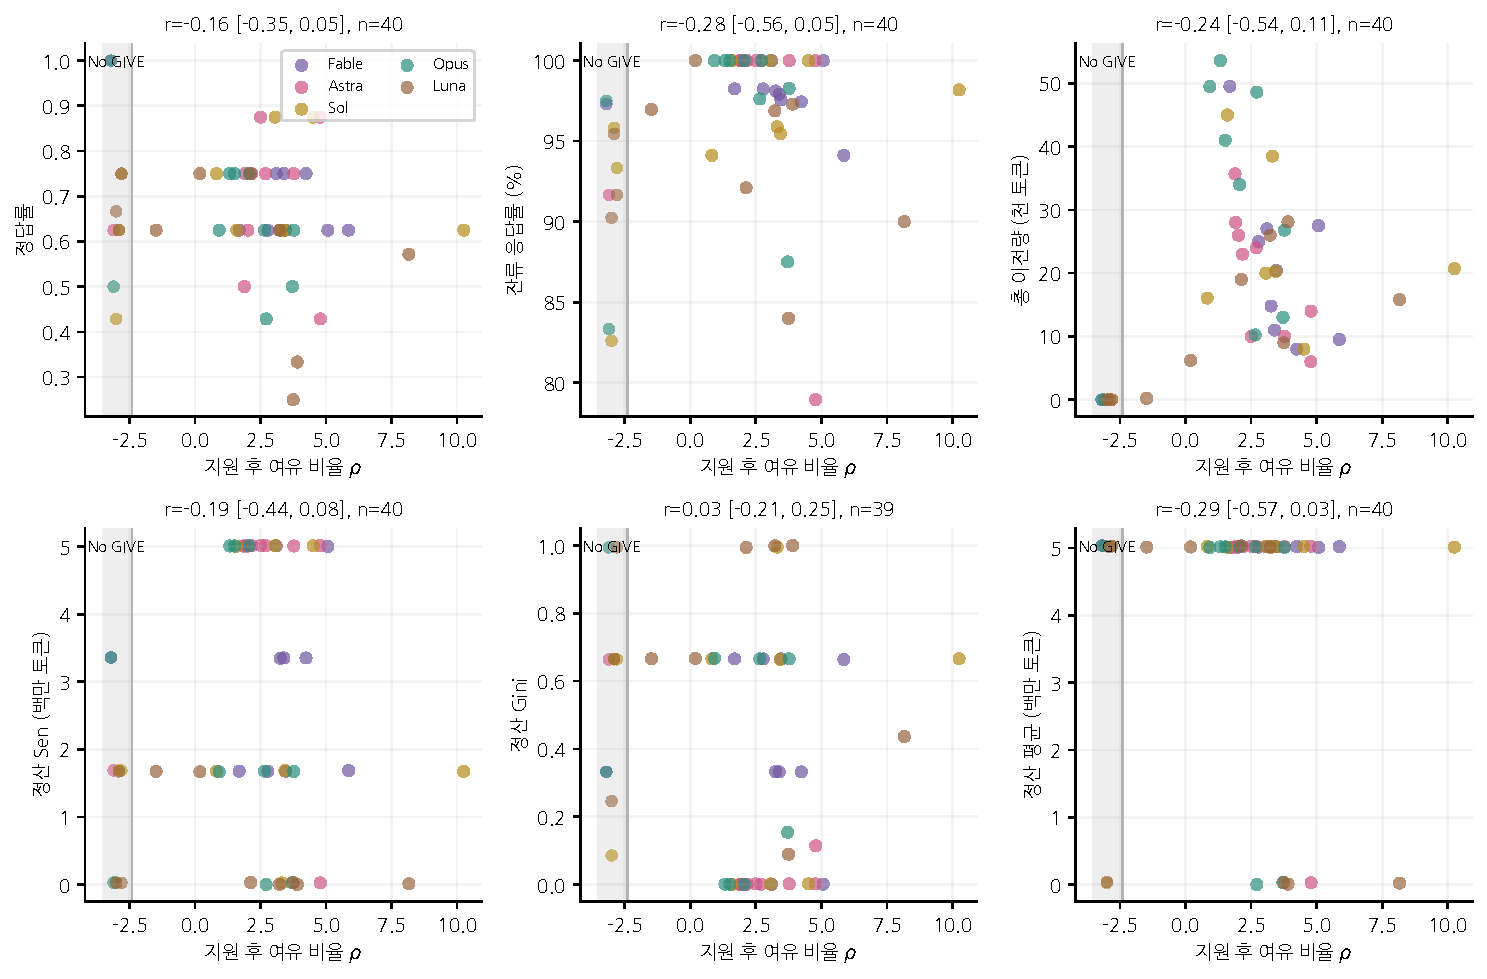
\includegraphics[width=\textwidth]{cogsci2027/ko/figures/appendix_refresh_20261107/rho_associations_10games.pdf}
\caption{판별 지원 후 여유 비율과 정답률, 잔류 응답률, 총 이전량 및 정산 자원 분포의 관계. 점 하나는 한 판이고 색은 모델이다. GIVE가 있었던 40판을 수치 축에 놓았으며 정산 Gini는 전원 잔액이 0인 한 판을 제외한 39판이다. GIVE가 없던 10판은 별도 No GIVE 띠에 놓았다. 이 띠의 위치는 여유 비율의 수치가 아니다. 제목은 Pearson 상관과 같은 시드의 다섯 모델을 묶어 2,000회 재표집한 백분위 95\% 구간이며 다중 비교 보정은 하지 않았다.}
\label{previous:fig:completion28-associations}
\end{figure}
